\documentclass{standalone}

\usepackage{tikz}

\begin{document}
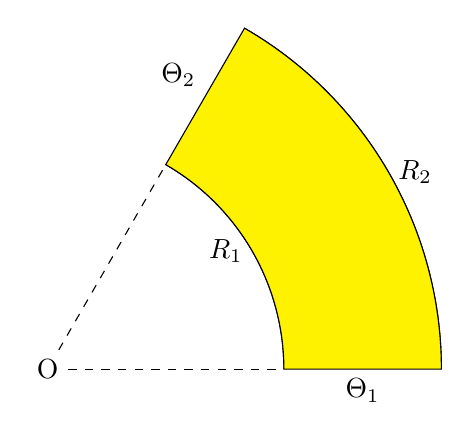
\begin{tikzpicture}
  \draw (0, 0) node (o) {O};
  \draw (3, 0) coordinate (r1start) {};
  \draw (5, 0) coordinate (r2start) {};
  \draw (60:3) coordinate (r1end) {};
  \draw (60:5) coordinate (r2end) {};
  \draw (r1start) arc (0:60:3);
  \draw (r2start) arc (0:60:5);
  \draw (30:3) node[anchor=east] (){$R_1$};
  \draw (30:5) node[anchor=west] (){$R_2$};
  \draw [dashed] (o) -- (r1start);
  \draw [dashed] (o) -- (r1end);
  \filldraw[fill=yellow] (r1start) arc (0:60:3) -- node[anchor=south east]{$\Theta_2$} (r2end) arc (60:0:5) -- node[anchor=north]{$\Theta_1$} cycle;
\end{tikzpicture}
\end{document}

%%% Local Variables:
%%% mode: latex
%%% TeX-master: t
%%% End:
